\phantomsection
\section*{六、CEC中的 LLM Inference Task Offloading}
\addcontentsline{toc}{section}{六、CEC中的 LLM Inference Task Offloading}

传统 CEC 计算卸载通常将任务建模为具有给定输入数据量、计算量、deadline 和能耗约束的计算 job，其核心问题是在本地设备、邻居设备、边缘服务器和云端之间选择执行位置，并联合优化通信资源和计算资源分配。在这一范式下，任务卸载的主要决策对象通常是完整任务、子任务、任务链断点或 DAG 节点，优化目标也多集中在时延、能耗、系统成本和队列稳定性等方面。


LLM inference task 改变了这一问题形态。与普通计算任务不同，LLM 推理的执行时间不仅由输入 prompt 决定，还受到输出长度、decode step 数、batch 状态、模型队列和上下文长度影响；一次请求也不一定只由单个模型独立完成，而可能需要多个模型、多个 agent、多个工具或多个 verifier 协作完成；多轮对话和长上下文服务则进一步引入 KV cache、prefix cache、session state、agent memory 和 user context 等运行时状态。因此，在 CEC 场景下，LLM inference task offloading 不再只是决定“一个任务是否卸载到边缘”，而是需要决定完整请求如何路由、多个模型或 agent 如何编排，以及支撑后续推理的 context/KV/runtime state 如何迁移、复用或重新计算。


基于上述特性，本章从一次 LLM 服务请求在 CEC 系统中的执行过程出发组织相关工作。具体而言，当一个 LLM request 到达系统后，首先需要决定该请求或会话应由哪个设备、边缘节点、云端服务或模型实例处理；对于复杂请求，系统可能进一步需要编排多个模型、agent 或工具形成协作式工作流；在请求执行和多轮交互过程中，context、KV cache、prefix cache、session state 和 agent memory 等运行时状态还需要在不同节点之间保留、迁移、复用或重新计算。因此，本章将现有方法划分为三类：request/session-level routing and offloading、multi-model/multi-agent workflow orchestration，以及 context/KV/runtime state offloading and migration，三类代表性工作分别在表~\ref{tab:request-session-routing}、表~\ref{tab:workflow-orchestration} 和表~\ref{tab:runtime-state-offloading} 中展开。

\textbf{代表工作总览。} 表~\ref{tab:cec-offloading-overview} 汇总了 LLM inference task offloading 相关工作的主归属、相关机制和方法关键词。前三类对应本章 6.1--6.3 的文献脉络，最后一类面向项目场景，将 request routing、KV/state management、SLA/memory 约束和长期 session cost 放入同一决策闭环。
\begingroup
\scriptsize
\setlength{\tabcolsep}{1.4pt}
\renewcommand{\arraystretch}{1.35}
\emergencystretch=2em
\begin{longtable}{@{}>{\raggedright\arraybackslash\hspace{0pt}}p{0.035\textwidth} >{\raggedright\arraybackslash\hspace{0pt}}p{0.175\textwidth} >{\raggedright\arraybackslash\hspace{0pt}}p{0.095\textwidth} >{\raggedright\arraybackslash\hspace{0pt}}p{0.170\textwidth} >{\raggedright\arraybackslash\hspace{0pt}}p{0.155\textwidth} >{\raggedright\arraybackslash\hspace{0pt}}p{0.330\textwidth}@{}}
\caption{\textbf{CEC 下 LLM Inference Task Offloading 代表工作总览}}
\label{tab:cec-offloading-overview}\\
\toprule
\textbf{序号} & \textbf{代表工作} & \textbf{发表在哪} & \textbf{主归属} & \textbf{相关机制} & \textbf{方法关键词} \\
\midrule
1 & QoS-LLM-Router \refcite{55} & TMC 2025 & Request / Session-level Routing and Offloading & QoS-aware routing；state-aware scheduling & 结合请求质量、响应长度、GPU memory 和队列状态，将 edge LLM expert routing 建模为长期 QoS 优化问题 \\
\tabrowrule
2 & CES-CB \refcite{56} & TSC 2025 & Request / Session-level Routing and Offloading & request cost prediction；combinatorial bandit & 利用 prompt embedding 和历史执行数据预测请求成本，在 edge/cloud 之间选择可提升吞吐并缓解长请求阻塞的请求集合 \\
\tabrowrule
3 & RouteLLM \refcite{57} & ICLR 2025 & Request / Session-level Routing and Offloading & strong/weak model routing & 基于 query 难度和偏好数据判断是否调用强模型，在保持质量的同时降低强模型调用成本 \\
\tabrowrule
4 & Training-Free Router \refcite{58} & NeurIPS 2025 & Request / Session-level Routing and Offloading & budget-aware multi-LLM routing & 通过近邻检索估计不同 LLM 的质量和成本，并用预算影子价格实现低训练成本的在线模型路由 \\
\tabrowrule
5 & ActiveInfer-Offload \refcite{59} & TMC 2024 & Request / Session-level Routing and Offloading & offloading；resource allocation & 使用 active inference 在不确定 cloud-edge 环境中联合决定 LLM inference task offloading 和资源分配 \\
\tabrowrule
6 & SLM-LLM-Collab \refcite{60} & TMC 2026 & Request / Session-level Routing and Offloading & SLM caching；D2D / edge collaboration & 在本地 SLM、邻居 SLM 和 edge LLM 之间做短时卸载决策，并将长期 SLM caching 作为请求路由前置条件 \\
\tabrowrule
7 & MGCO \refcite{61} & TSC 2026 & Request / Session-level Routing and Offloading & mobility-aware offloading & 用 Transformer MHA encoder 建模历史决策和未来移动状态，使 generative computation offloading 避免短视路由 \\
\tabrowrule
8 & MasRouter \refcite{62} & ACL 2025 & Multi-model / Multi-agent Workflow Orchestration & multi-agent routing & 联合选择协作模式、agent 数量、角色分工和底层 LLM，使 multi-agent system configuration 匹配 query 难度 \\
\tabrowrule
9 & Conductor \refcite{63} & ICLR 2026 & Multi-model / Multi-agent Workflow Orchestration & natural-language workflow control & 训练元控制器用自然语言生成多模型 workflow，控制 subtask、model id 和上下文访问范围 \\
\tabrowrule
10 & AFLOW \refcite{64} & ICLR 2025 & Multi-model / Multi-agent Workflow Orchestration & automatic agentic workflow search & 将 agentic workflow 表示为代码形式的 LLM 调用图，通过搜索和执行反馈自动优化复杂任务 workflow \\
\tabrowrule
11 & DT-MADTO \refcite{65} & TMC 2025 & Multi-model / Multi-agent Workflow Orchestration & mobility-aware DAG offloading & 用 digital twin 预测移动和资源状态，联合决策 DAG 子任务卸载、带宽分配和中间数据等待时间 \\
\tabrowrule
12 & FuseSpill \refcite{66} & TPDS 2026 & Context / KV / Runtime State Offloading and Migration & KV spillover；auxiliary GPU scheduling & 在显存受限 GPU 上按代价模型选择 KV cache 溢出策略，并将溢出序列调度到辅助 GPU 继续 decode \\
\tabrowrule
13 & Weaver \refcite{67} & USENIX ATC 2025 & Context / KV / Runtime State Offloading and Migration & attention offloading & 通过 attention offloading 缓解 multi-LLM serving 中的资源压力，提高多模型服务吞吐和资源利用率 \\
\tabrowrule
14 & Mooncake \refcite{21} & USENIX FAST 2025 & Context / KV / Runtime State Offloading and Migration & distributed KV cache；global scheduling & 将 CPU/DRAM/SSD/RDMA 组织为全局 KVCache Store，并按缓存命中、节点负载和 TTFT/TBT SLO 调度请求 \\
\tabrowrule
15 & CA-AIGC-Migration \refcite{69} & TSC 2026 & Context / KV / Runtime State Offloading and Migration & context migration；mobility-aware service migration & 将模型迁移转化为 context migration，在 reward 中联合考虑 context relevance、AoI、计算延迟和传输成本 \\
\tabrowrule
16 & 长期成本感知请求卸载方案 & 本报告 & Project-oriented Long-term Cost-aware Offloading & mobility/length prediction；action masking；block-level KV management & 联合选择计算节点与 KV reuse/sync/recompute 方式，在满足 P99 E2E latency 和 memory 约束下最小化 session 长期服务成本 \\
\bottomrule
\end{longtable}
\endgroup




\phantomsection
\subsection*{6.1 Request / Session-level Routing and Offloading}
\addcontentsline{toc}{subsection}{6.1 Request / Session-level Routing and Offloading}

Request/session-level routing 是最接近传统 task offloading 的 LLM inference offloading 形式。它将完整 LLM 请求、query、conversation turn 或 session 作为基本决策对象，决定其应该由本地设备、邻居设备、接入边缘、区域边缘还是云端服务处理。与普通任务不同，LLM request 的处理时间往往难以在执行前准确确定，因为它不仅取决于 prompt length，还受到 output length、decode step 数、batch 状态和模型当前队列影响。对于多个 edge LLM experts、多个 SLM/LLM 服务或多层 device-edge-cloud 网络，系统还需要根据请求复杂度、模型能力、响应质量、时延约束、GPU memory、队列状态和云端成本进行联合决策。


这一类问题的核心矛盾是：edge 具有低时延、低回传开销和隐私优势，但计算资源和显存有限，长输出请求可能占据 batch 并造成 head-of-line blocking；cloud 算力充足且模型能力更强，但会带来更高 RTT、带宽开销和数据出域风险。对于 CEC 系统而言，请求路由不应只回答“是否卸载到边缘”，还需要回答“卸载到哪个 edge server”“调用哪个 LLM expert”“是否先由 SLM 处理”“是否需要递归升级到更强模型或云端模型”等问题。表~\ref{tab:request-session-routing} 汇总了该方向的代表性工作。


\begin{table}[!htbp]
    \centering
    \caption{\textbf{Request / Session-level Routing and Offloading 代表性工作}}
    \label{tab:request-session-routing}
    \renewcommand{\arraystretch}{1.45}
    \scriptsize
    \setlength{\tabcolsep}{4pt}
    \begin{tabularx}{\textwidth}{@{}>{\hsize=0.75\hsize\raggedright\arraybackslash}X >{\hsize=0.75\hsize\raggedright\arraybackslash}X >{\hsize=1.15\hsize\raggedright\arraybackslash}X >{\hsize=1.15\hsize\raggedright\arraybackslash}X >{\hsize=1.20\hsize\raggedright\arraybackslash}X@{}}
        \toprule
        \textbf{代表工作} & \textbf{发表在哪 \& 时间} & \textbf{问题表述} & \textbf{核心方法} & \textbf{优化目标} \\
        \midrule
        QoS-LLM-Router \refcite{55} & TMC, 2025 & 多个 edge LLM experts 在生成质量、响应长度、GPU memory 和队列状态上异构；动态到达的请求需要实时选择 expert，以同时保证 response quality 和 latency requirement。 & 将请求路由建模为 infinite-horizon MDP；使用 DistilBERT-based predictors 预测 response quality 和 length；使用 heterogeneous graph attention network 抽象系统状态，并用 SAC 学习 QoS-aware routing policy。 & 最大化长期 accumulated QoS，同时考虑 response quality 和 latency constraint。 \\
        \tabrowrule
        CES-CB \refcite{56} & TSC, 2025 & LLM request 的 output length 和处理时间不可预测；如果长请求留在 edge，会阻塞后续短请求并降低 edge throughput。 & 将 prompt embedding 作为 context，将每轮 edge batch selection 建模为 contextual combinatorial semi-bandit；使用 neural prediction 与 UCB 机制平衡 exploration/exploitation。 & 最大化 edge throughput，减少因长请求导致的 head-of-line blocking。 \\
        \tabrowrule
        RouteLLM \refcite{57} & ICLR, 2025 & 给定一个 query，如何在推理前决定调用强模型还是弱模型，使系统在满足质量目标的同时尽量少调用强模型。 & 使用偏好数据训练 router，预测强模型相比弱模型是否具有明显优势；根据阈值决定调用强模型还是弱模型。 & 在保持回复质量的同时降低强模型调用比例和推理成本。 \\
        \tabrowrule
        Training-Free Router \refcite{58} & NeurIPS, 2025\newline  & 在高流量、多 LLM 在线服务中，如何在不知道未来请求、预算有限且不能频繁训练 router 的情况下，快速把每个 query 分配给最合适的 LLM，以最大化整体回答质量并控制成本。 & 先用历史 query 的近邻检索（ANNS）快速估计当前 query 在各个 LLM 上的质量和成本，再用最开始一小部分在线 query 做一次轻量优化，学习每个 LLM 的预算“影子价格” $\gamma$。之后每个新 query 只需按 “估计质量收益 − 预算成本惩罚” 打分，选择得分最高的 LLM，从而实现无需训练、低延迟、预算感知的在线路由。 & 在每个 LLM 的 token 预算约束下，为在线到达的 queries 选择路由模型，使所有已处理 queries 的总体回答质量/性能最大化。 \\
        \tabrowrule
        ActiveInfer-Offload \refcite{59} & TMC, 2024 & Cloud-edge LLM inference 需要同时考虑任务卸载和资源分配；传统 DRL 方法数据效率低，且难以适应动态任务负载和 latency requirement。 & 使用 active inference 框架建模 LLM inference task offloading 和 resource allocation，在不确定环境下进行在线决策。 & 优化 cloud-edge LLM inference 的服务性能、资源利用和时延表现。 \\
        \tabrowrule
        SLM-LLM-Collab \refcite{60} & TMC, 2026 & 在给定 SLM/LLM 服务能力和缓存状态下，每个请求需要决定本地 SLM 执行、D2D 卸载给邻居 SLM，还是卸载到 edge LLM 与 cached SLM plugins 协同推理。 & 在短时间尺度上使用 factor graph 和 belief propagation 进行分布式 inference offloading 决策；长期 SLM caching 部分作为请求路由的前置条件，而非本节重点。 & 在时延和显存约束下最大化长期平均推理准确率。 \\
        \tabrowrule
        MGCO \refcite{61} & TSC, 2026 & 移动场景下，generative computation offloading action 会受到历史决策和未来移动状态影响；短程决策容易短视，且传统 RNN/LSTM 对长序列建模能力有限。 & 使用 Transformer MHA encoder 建模长程移动和历史决策信息；通过候选移动区域约束缩减 action space，提高收敛效率。 & 在移动 edge-cloud 系统中实现更高效的 generative computation offloading，降低长期服务开销。 \\
        \bottomrule
    \end{tabularx}
\end{table}


从 CEC 角度看，上述工作共同说明，LLM request routing 不能简单沿用传统 task offloading 中“输入数据量 + CPU cycles + deadline”的建模方式。一方面，请求执行时间受到输出长度和 batch 状态影响，具有更强的不确定性；另一方面，请求质量取决于模型能力、prompt 语义和模型选择，而不是单纯取决于计算资源是否充足。因此，CEC 中的 request-level offloading 需要同时感知 semantic complexity、model capability、network condition 和 queue state。


多用户和移动性会进一步放大这一复杂性。用户位置变化会改变接入边缘、链路质量、候选服务节点和区域请求热点；请求执行过程中可能发生 handover，多轮会话的 context 或 KV cache 也可能留在旧 edge。因此，request/session routing 不能只根据当前时隙的队列和链路状态做短视选择，而需要同时考虑未来位置变化、会话连续性、状态位置和模型可用性。未来可以进一步研究 mobility-aware session routing，使请求路径选择同时感知用户移动趋势、后续多轮会话、模型缓存位置和 context/KV 可复用性。




\phantomsection
\subsection*{6.2 Multi-model / Multi-agent Workflow Orchestration}
\addcontentsline{toc}{subsection}{6.2 Multi-model / Multi-agent Workflow Orchestration}

随着 LLM 从单轮问答走向复杂推理、代码生成、工具调用、科学问答和长期任务执行，一个 request 到来后，系统不一定只调用一个模型完成回答。更一般的形式是：系统根据请求复杂度和任务类型，动态选择多个模型、多个 agent 或多个工具，并决定它们之间的角色分工、通信拓扑、执行顺序、上下文可见性和结果聚合方式。这一类问题可以被称为 multi-model 或 multi-agent workflow orchestration。


这一类问题与传统 stage-level offloading 或 splittable-request offloading 不同。Stage-level offloading 关注 prefill、decode、verification、diffusion steps 等底层执行阶段如何分布到不同计算节点；而 multi-agent workflow orchestration 关注的是语义层和任务层的协作结构，例如是否需要 planner、solver、critic、verifier、researcher、programmer 等角色，是否采用 Chain-of-Thought、Self-Consistency、LLM Debate、chain topology 或 complete graph 等协作模式，以及每个 agent 背后调用哪个 LLM 或 SLM。换言之，这里的决策对象不是 token、模型层或推理阶段，而是一个 request 的 problem-solving workflow。


这一类问题的核心矛盾是：多 agent 协作可以提升复杂任务的推理能力、鲁棒性和可解释性，但也会带来额外模型调用成本、通信开销、上下文传输开销和调度复杂度。对于 CEC 系统而言，agent 背后的模型、工具、数据库、memory 和 verifier 可能分布在用户设备、边缘服务器、区域云和中心云上。因此，multi-agent workflow orchestration 不仅是算法层的协作模式选择问题，也是计算、通信、状态和隐私的联合编排问题。表~\ref{tab:workflow-orchestration} 列出了相关代表性工作。


\begin{table}[!htbp]
    \centering
    \caption{\textbf{Multi-model / Multi-agent Workflow Orchestration 代表性工作}}
    \label{tab:workflow-orchestration}
    \renewcommand{\arraystretch}{1.45}
    \scriptsize
    \setlength{\tabcolsep}{4pt}
    \begin{tabularx}{\textwidth}{@{}>{\hsize=0.75\hsize\raggedright\arraybackslash}X >{\hsize=0.75\hsize\raggedright\arraybackslash}X >{\hsize=1.15\hsize\raggedright\arraybackslash}X >{\hsize=1.15\hsize\raggedright\arraybackslash}X >{\hsize=1.20\hsize\raggedright\arraybackslash}X@{}}
        \toprule
        \textbf{代表工作} & \textbf{发表在哪 \& 时间} & \textbf{问题表述} & \textbf{核心方法} & \textbf{优化目标} \\
        \midrule
        RouteLLM \refcite{57} & ICLR, 2025 & 现有 LLM serving 中，所有 query 都调用强模型会带来高成本，而固定使用弱模型又可能损害回答质量；需要根据 query 难度选择合适模型。 & 使用偏好数据训练一个 query-level router，预测强模型是否会显著优于弱模型；根据阈值进行强/弱模型选择。 & 在保持目标回答质量的同时减少强模型调用比例，降低推理成本。 \\
        \tabrowrule
        MasRouter \refcite{62} & ACL, 2025 & 现有 LLM routing 多解决“给单个 agent 选哪个 LLM”的问题，但在多智能体系统中，真正需要 routing 的还包括协作模式、agent 数量、角色分工以及每个角色对应的底层 LLM。 & 通过将 query 映射到 latent space 选择合作模式和 agent 数量；使用 structured probabilistic cascade 为 agent 分配角色；再用多项分布为每个角色选择底层 LLM；训练时使用 policy gradient 优化。 & 为每个 query 选择合适的 multi-agent system configuration，使回复质量和准确率尽可能高，同时控制推理成本。 \\
        \tabrowrule
        Conductor \refcite{63} & ICLR, 2026\newline  & 如何训练一个元控制器，让它用自然语言自动编排多个已有 LLM，使整体系统超过任一单个 worker。 & 使用一个 SLM 作为 Conductor，根据 query 生成自然语言 workflow；每个 step 包含 subtask、model id 和 access list；训练阶段采样多个 candidate workflows，根据最终答案正确性给 reward，并用 GRPO 更新 Conductor。 & 让 Conductor 学会任务拆解、模型选择、上下文可见性控制和 workflow 生成，使多模型协作后的最终答案尽可能正确。 \\
        \tabrowrule
        AFLOW \refcite{64} & ICLR, 2025 & 如何在尽量减少人工设计的情况下，自动生成并优化由多次 LLM 调用组成的 agentic workflow，从而提升 LLM 在问答、代码生成和数学推理等复杂任务上的表现。 & AFLOW 将 agentic workflow 表示为代码形式的 LLM 调用图/流程，并把 workflow 优化转化为一个搜索问题。选择已有高分 workflow，让 LLM 修改 prompt 或代码结构生成新 workflow，再执行评估，并把成功/失败经验回传到搜索树中，从而逐步找到更优工作流。 & 给定任务 T 和评价函数 G，在所有可能的 workflow 中找到使任务表现 G(W,T) 最大的工作流 W\newline  \\
        \tabrowrule
        DT-MADTO \refcite{65} & TMC, 2025\newline  & 移动用户产生具有 DAG 依赖关系的复杂任务；设备移动导致链路状态和中间数据流传输代价动态变化，同时多设备并发卸载会造成 flow congestion。 & 构建 device、physical CEC、digital twin 三层架构；使用 digital twin 预测未来移动和资源状态，并用 DDPG / actor-critic 联合决策 subtask offloading、bandwidth allocation 和 flow waiting time。 & 最小化任务完成时间和能耗的加权 QoS 指标。 \\
        \bottomrule
    \end{tabularx}
\end{table}


从 LLM serving 角度看，RouteLLM 可以被视为 multi-agent routing 的基础形式：它只在强模型和弱模型之间做 query-level routing，尚未涉及 agent 数量、角色分配或协作拓扑。MasRouter 则进一步把 routing 扩展到 multi-agent system configuration，即根据 query 决定采用哪种协作模式、需要多少个 agent、每个 agent 扮演什么角色，以及每个角色调用哪个底层 LLM。Conductor 更进一步，不再只在预定义配置集合中选择，而是训练一个控制器用自然语言生成 workflow，包括任务拆解、模型调用和上下文访问控制。AFLOW则是将workflow表示为代码形式，通过搜索方法，实时根据当前任务执行情况自适应生成新的workflow。


从 CEC 角度看，multi-agent workflow orchestration 需要被进一步物理化。现有 multi-agent orchestration 工作大多默认所有 worker LLM 都可以通过 API 调用，较少考虑模型、工具和 memory 的实际部署位置。但在 CEC 系统中，不同 agent 可能对应不同物理节点：本地设备上的 SLM 可以承担隐私敏感的初步理解任务，近端 edge 上的 LLM 可以承担低时延交互任务，区域边缘或云端的大模型可以承担复杂推理和 verification 任务，外部工具或数据库 agent 也可能位于不同网络位置。因此，agent workflow 的拓扑会直接影响端到端时延、带宽消耗、隐私风险和状态迁移成本。


多用户移动性进一步使 multi-agent workflow orchestration 变得更复杂。用户移动会改变可访问的 edge agents、工具服务和 memory 节点；workflow 中间状态可能在多个 agent 之间传递，如果用户在执行过程中发生 handover，后续 agent 是否继续在旧 edge 执行、是否迁移到新 edge、是否远程访问旧 context，都会影响服务质量。虽然 DT-MADTO \refcite{65} 并不是 LLM agent workflow 工作，但其对 DAG 依赖关系、中间数据流和移动预测的建模，为 CEC 中的 multi-agent workflow offloading 提供了可借鉴思路。未来可以进一步研究 mobility-aware agent workflow orchestration，在 request 到达时联合决定协作模式、agent 位置、模型选择、上下文可见性和中间状态传输路径。




\phantomsection
\subsection*{6.3 Context / KV / Runtime State Offloading and Migration}
\addcontentsline{toc}{subsection}{6.3 Context / KV / Runtime State Offloading and Migration}

LLM inference 与普通计算任务的另一个关键区别在于运行时状态会持续影响后续请求。多轮对话、长上下文服务、prefix reuse 和 agent workflow 会产生 KV cache、prefix cache、session state、agent memory、tool outputs 和 intermediate reasoning traces。这些状态的位置会直接影响后续 TTFT、decode latency、重复计算成本、跨节点传输开销、隐私边界和服务连续性。因此，context/KV/runtime state offloading 关注的不是计算任务本身去哪执行，而是支撑后续推理的状态应该保留在哪里、何时迁移、是否远程访问、是否复用或是否重新计算。


这一类问题的核心矛盾是：状态迁移可以保持多轮服务连续性、减少重复 prefill 计算并提升生成质量；但迁移或远程访问状态会消耗带宽、显存和存储资源，也可能增加一致性管理和隐私风险。对于长上下文 chatbot，KV cache 和 prefix cache 可能比单次请求本身更有价值；对于 multi-agent workflow，中间结果、工具调用结果和 agent memory 也可能在后续步骤或后续会话中被反复使用。因此，LLM inference offloading 的优化目标正在从 computation-aware 转向 computation-state co-optimization。表~\ref{tab:runtime-state-offloading} 汇总了 context、KV 和 runtime state 卸载迁移方向的代表性工作。


\begin{table}[!htbp]
    \centering
    \caption{\textbf{Context / KV / Runtime State Offloading and Migration 代表性工作}}
    \label{tab:runtime-state-offloading}
    \renewcommand{\arraystretch}{1.45}
    \scriptsize
    \setlength{\tabcolsep}{4pt}
    \begin{tabularx}{\textwidth}{@{}>{\hsize=0.75\hsize\raggedright\arraybackslash}X >{\hsize=0.75\hsize\raggedright\arraybackslash}X >{\hsize=1.15\hsize\raggedright\arraybackslash}X >{\hsize=1.15\hsize\raggedright\arraybackslash}X >{\hsize=1.20\hsize\raggedright\arraybackslash}X@{}}
        \toprule
        \textbf{代表工作} & \textbf{发表在哪 \& 时间} & \textbf{问题表述} & \textbf{核心方法} & \textbf{优化目标} \\
        \midrule
        FuseSpill \refcite{66} & TPDS, 2026 & 在显存受限 GPU 上进行 LLM 推理时，KV cache 容易溢出，现有 swap/recompute 策略处理低效，导致吞吐下降和溢出请求延迟增加。 & FuseSpill 通过代价模型自适应选择 KV cache 溢出策略，并把溢出或主动卸载的序列调度到辅助 GPU 继续 decode，从而释放主 GPU 显存、提高 prefill/decode 利用率。 & 在显存受限 GPU 上提高 LLM 推理吞吐量，同时降低发生 KV cache spillover 的请求延迟。 \\
        \tabrowrule
        Weaver \refcite{67} & USENIX ATC, 2025 & 多 LLM serving 中 attention computation 和模型实例管理会造成资源压力；attention 和相关状态如何 offload 会影响多模型服务效率。 & 通过 attention offloading 提升 multi-LLM serving 的资源效率，并缓解多模型服务中的资源压力。 & 提高多模型服务吞吐和资源利用率。 \\
        \tabrowrule
        Mooncake \refcite{21} & USENIX FAST, 2025 & 在长上下文 LLM 聊天服务中，如何用全局分布式 KV cache 复用历史前缀计算，减少昂贵的 prefill GPU 计算，从而在满足 TTFT/TBT 延迟要求的同时提升系统吞吐。 & 把 LLM 推理拆成 prefill 和 decoding 两个独立资源池，并把集群中 CPU/DRAM/SSD/RDMA 组织成全局分布式 KVCache Store；调度器根据缓存命中、节点负载和 TTFT/TBT SLO，把请求路由到合适的 prefill/decoding 节点。 & 用更多存储换取更少重复计算，提高长上下文 LLM serving 效率。 \\
        \tabrowrule
        DistServe \refcite{7} & USENIX OSDI, 2024 & Prefill 和 decode 混部执行会造成阶段间干扰，并耦合两阶段资源分配；两阶段分离后，KV handoff 和状态传输成为连接 prefill 与 decode 的关键问题。 & 将 prefill 和 decoding 分离到不同 worker/resource pool，并根据 TTFT/TPOT 需求分别优化资源分配和并行策略。 & 最大化满足 TTFT 和 TPOT 约束下的 goodput。 \\
        \tabrowrule
        T2DRL \refcite{68} & TON, 2026 & Mobile edge 难以支撑 long-context LLM agents 的多轮交互，因为 context window 会同时影响准确率、延迟和资源消耗；模型缓存和请求执行策略需要随上下文和使用模式变化。 & 提出 T2DRL 框架，在训练和测试阶段共同学习 cached models 与 service requests 的管理策略，并结合 double Dutch auction 做资源匹配。 & 降低系统成本，同时保证 long-context LLM agents 在感知和推理任务中的服务性能。 \\
        \tabrowrule
        CA-AIGC-Migration \refcite{69} & TSC, 2026\newline  & 用户移动到新边缘节点后，旧节点上的 long context 是有价值但迁移成本较高的状态资产；传统 service migration 迁移完整模型成本过高。 & 利用 LLM in-context learning 特性，将 model migration 转化为 context migration；在 reward 中联合考虑 context relevance、AoI、计算延迟和传输成本，并用 Transformer DRL 学习迁移策略。 & 在保持 AIGC 回复质量和准确性的同时降低 context migration 成本和服务时延。 \\
        \bottomrule
    \end{tabularx}
\end{table}


从系统角度看，KV cache、prefix cache 和 context 不再只是 LLM inference 的内部实现细节，而是 CEC 中可以被 offload、cache、migrate 和 schedule 的重要资源。Mooncake 说明了长上下文服务中 KV cache 可以作为全局分布式存储资源被管理；DistServe 说明了 prefill/decode disaggregation 会使 KV handoff 成为连接不同资源池的关键状态传输；FuseSpill \refcite{66} 和 Weaver \refcite{67} 则从显存约束和 attention offloading 角度说明，runtime state 的位置会直接影响吞吐和时延。


在 CEC 中，context/KV/runtime state offloading 需要进一步考虑边缘节点之间的异构资源和网络差异。对于多轮会话，如果每轮请求都重新 prefill 长上下文，会产生大量重复计算；如果跨节点远程访问 KV cache，则会引入额外 RTT 和带宽开销；如果主动迁移 context 或 KV，则可能占用边缘链路和存储资源。因此，系统需要在远程访问、状态迁移、状态压缩、状态丢弃和重新计算之间进行选择。


多用户移动性使这一问题更加突出。用户移动后，计算路径可以重新选择，但 long context、KV cache、agent memory 或 session state 可能仍保留在旧 edge。此时系统需要在四种选择之间权衡：迁移状态到新 edge、远程访问旧状态、重新计算状态，或丢弃部分状态并降低上下文质量。不同选择会影响后续 decode latency、生成质量、带宽消耗和隐私边界。CA-AIGC-Migration \refcite{69} 已经开始从 context migration 的角度研究这一问题，但对 KV cache placement、remote KV access、prefix cache sharing 和 agent memory migration 的移动 CEC 场景研究仍然不足。未来可以进一步研究 mobility-aware KV and context management，将用户轨迹预测、session continuation probability、KV reuse probability、edge storage pressure 和链路状态联合纳入决策。








\phantomsection
\subsection*{6.4 面向项目场景的长期成本感知请求卸载方案}
\addcontentsline{toc}{subsection}{6.4 面向项目场景的长期成本感知请求卸载方案}

本项目包含三个部署相同模型的推理节点，每个节点既是请求入口，也是候选计算节点；两条链路为 100 Gbps，另一条为 25 Gbps。对于包含 \(K\) 个请求的 LLM session，系统在用户移动和输出长度未知的条件下，联合选择计算节点与 KV 获取方式，并在满足 E2E latency SLA 和显存约束的前提下最小化长期成本。

\textbf{主要符号。}
\begingroup
\small
\setlength{\LTpre}{4pt}
\setlength{\LTpost}{6pt}
\begin{longtable}{p{0.29\textwidth}p{0.65\textwidth}}
\toprule
符号 & 含义 \\
\midrule
\endfirsthead
\toprule
符号 & 含义 \\
\midrule
\endhead
\(k,K,\mathcal N\) & 当前请求编号、session 请求总数和候选节点集合 \\
\(i,j,n,s\) & 入口节点、目标/计算节点、一般节点和 KV 同步源节点索引 \\
\(U_k,J_k,\Delta\tau_k\) & 当前入口、所选计算节点和相邻请求间隔 \\
\(P_{ij}(\Delta\tau_k),b_k\) & 入口转移概率和多步移动预测分布 \\
\(x_k,Y_k,\rho_k(y),\widehat Y_k^{(p)}\) & 请求特征、实际输出长度、长度预测分布和第 \(p\) 分位预测 \\
\(\mathcal B_k,\mathcal B_{k,n}\) & 当前完整 KV block 集合和节点 \(n\) 已有 block 集合 \\
\(v_{k,n},\mathcal C_k\) & 节点 \(n\) 的最高连续 KV 版本和版本化多副本状态 \\
\(\mathcal M_{k,j},q_b,\Delta\mathcal B_k\) & 节点 \(j\) 缺失 blocks、block \(b\) 的大小和本轮新增 blocks \\
\(\psi_k^{\mathrm{cache}}\) & KV 副本保留与驱逐策略 \\
\(a_k=(J_k,Z_k)\) & 计算节点与 KV 获取方式组成的联合动作 \\
\(Z_k\) & KV 获取方式：\(\mathrm{reuse}\)、\(\mathrm{sync}\) 或 \(\mathrm{recompute}\) \\
\(\mathcal A_k^F(s_k)\) & 满足 SLA、显存、版本和节点可用性约束的动作集合 \\
\(D_k^{\mathrm{input}},D_k^{\mathrm{request}}\) & 输入数据量和跨节点请求/响应总字节数 \\
\(D_k^{\mathrm{KV}},BW_{i,j}^{\mathrm{eff}}\) & KV 同步字节数和节点间实测有效带宽 \\
\(L_k^{\mathrm{new}},L_k^{\mathrm{ctx}}\) & 未被 KV 覆盖的新输入长度和完整上下文长度 \\
\(\tau_j^{\mathrm{prefill}}(L)\) & 节点 \(j\) 处理 \(L\) 个 prefill tokens 的实测时间 \\
\(T_k^{\mathrm{comm}},T_k^{\mathrm{state}},T_k^{\mathrm{prefill}}\) & 请求通信、KV 状态准备和 prefill 时间 \\
\(T_k^{\mathrm{queue}},T_k^{\mathrm{decode}},T_k^{\mathrm{return}}\) & 排队、decode 和结果返回时间 \\
\(T_k^{\mathrm{E2E}}\) & 从请求发出到全部输出返回的端到端时延 \\
\(C_k^{\mathrm{eviction}},w_1,\ldots,w_4,c_k\) & KV 驱逐损失、成本权重和当前期望成本 \\
\(\Delta_k(a),SLA_k\) & 动作时延安全裕量和请求 SLA 上限 \\
\(\widehat M_k,M^{\mathrm{reserve}},M_{J_k}^{\mathrm{free}}\) & 预测显存需求、安全预留显存和计算节点剩余显存 \\
\(s_k,\mathbf L_k,\mathbf M_k,\mathbf W_k\) & 系统状态及其中的负载、显存和链路状态向量 \\
\(\pi,\gamma,\mathcal Q^*\) & 路由策略、折扣因子和最优状态--动作价值 \\
\(\mathcal Q_\theta,\mathcal Q_{\bar\theta}\) & Double DQN 在线网络和目标网络 \\
\(a_{k+1}^{\mathrm{sel}},V_{k+1},z_k\) & 下一动作选择、目标网络估值和 Bellman 训练目标 \\
\(\mathcal M^{\mathrm{mig}},\mathcal M^{\mathrm{rec}}\) & 混合 KV 恢复中迁移和重算的缺失 block 子集 \\
\(T^{\mathrm{mig}},T^{\mathrm{rec}},T^{\mathrm{hybrid}},T^{\mathrm{overhead}}\) & 迁移、重算、混合恢复和流水调度附加时间 \\
\bottomrule
\end{longtable}
\endgroup

图~\ref{fig:ch6-mobility-offloading-workflow} 给出了本方案从状态采集、预测、可行性过滤、长期路由到 KV 管理和在线反馈的完整流程。

\begin{figure}[H]
\centering
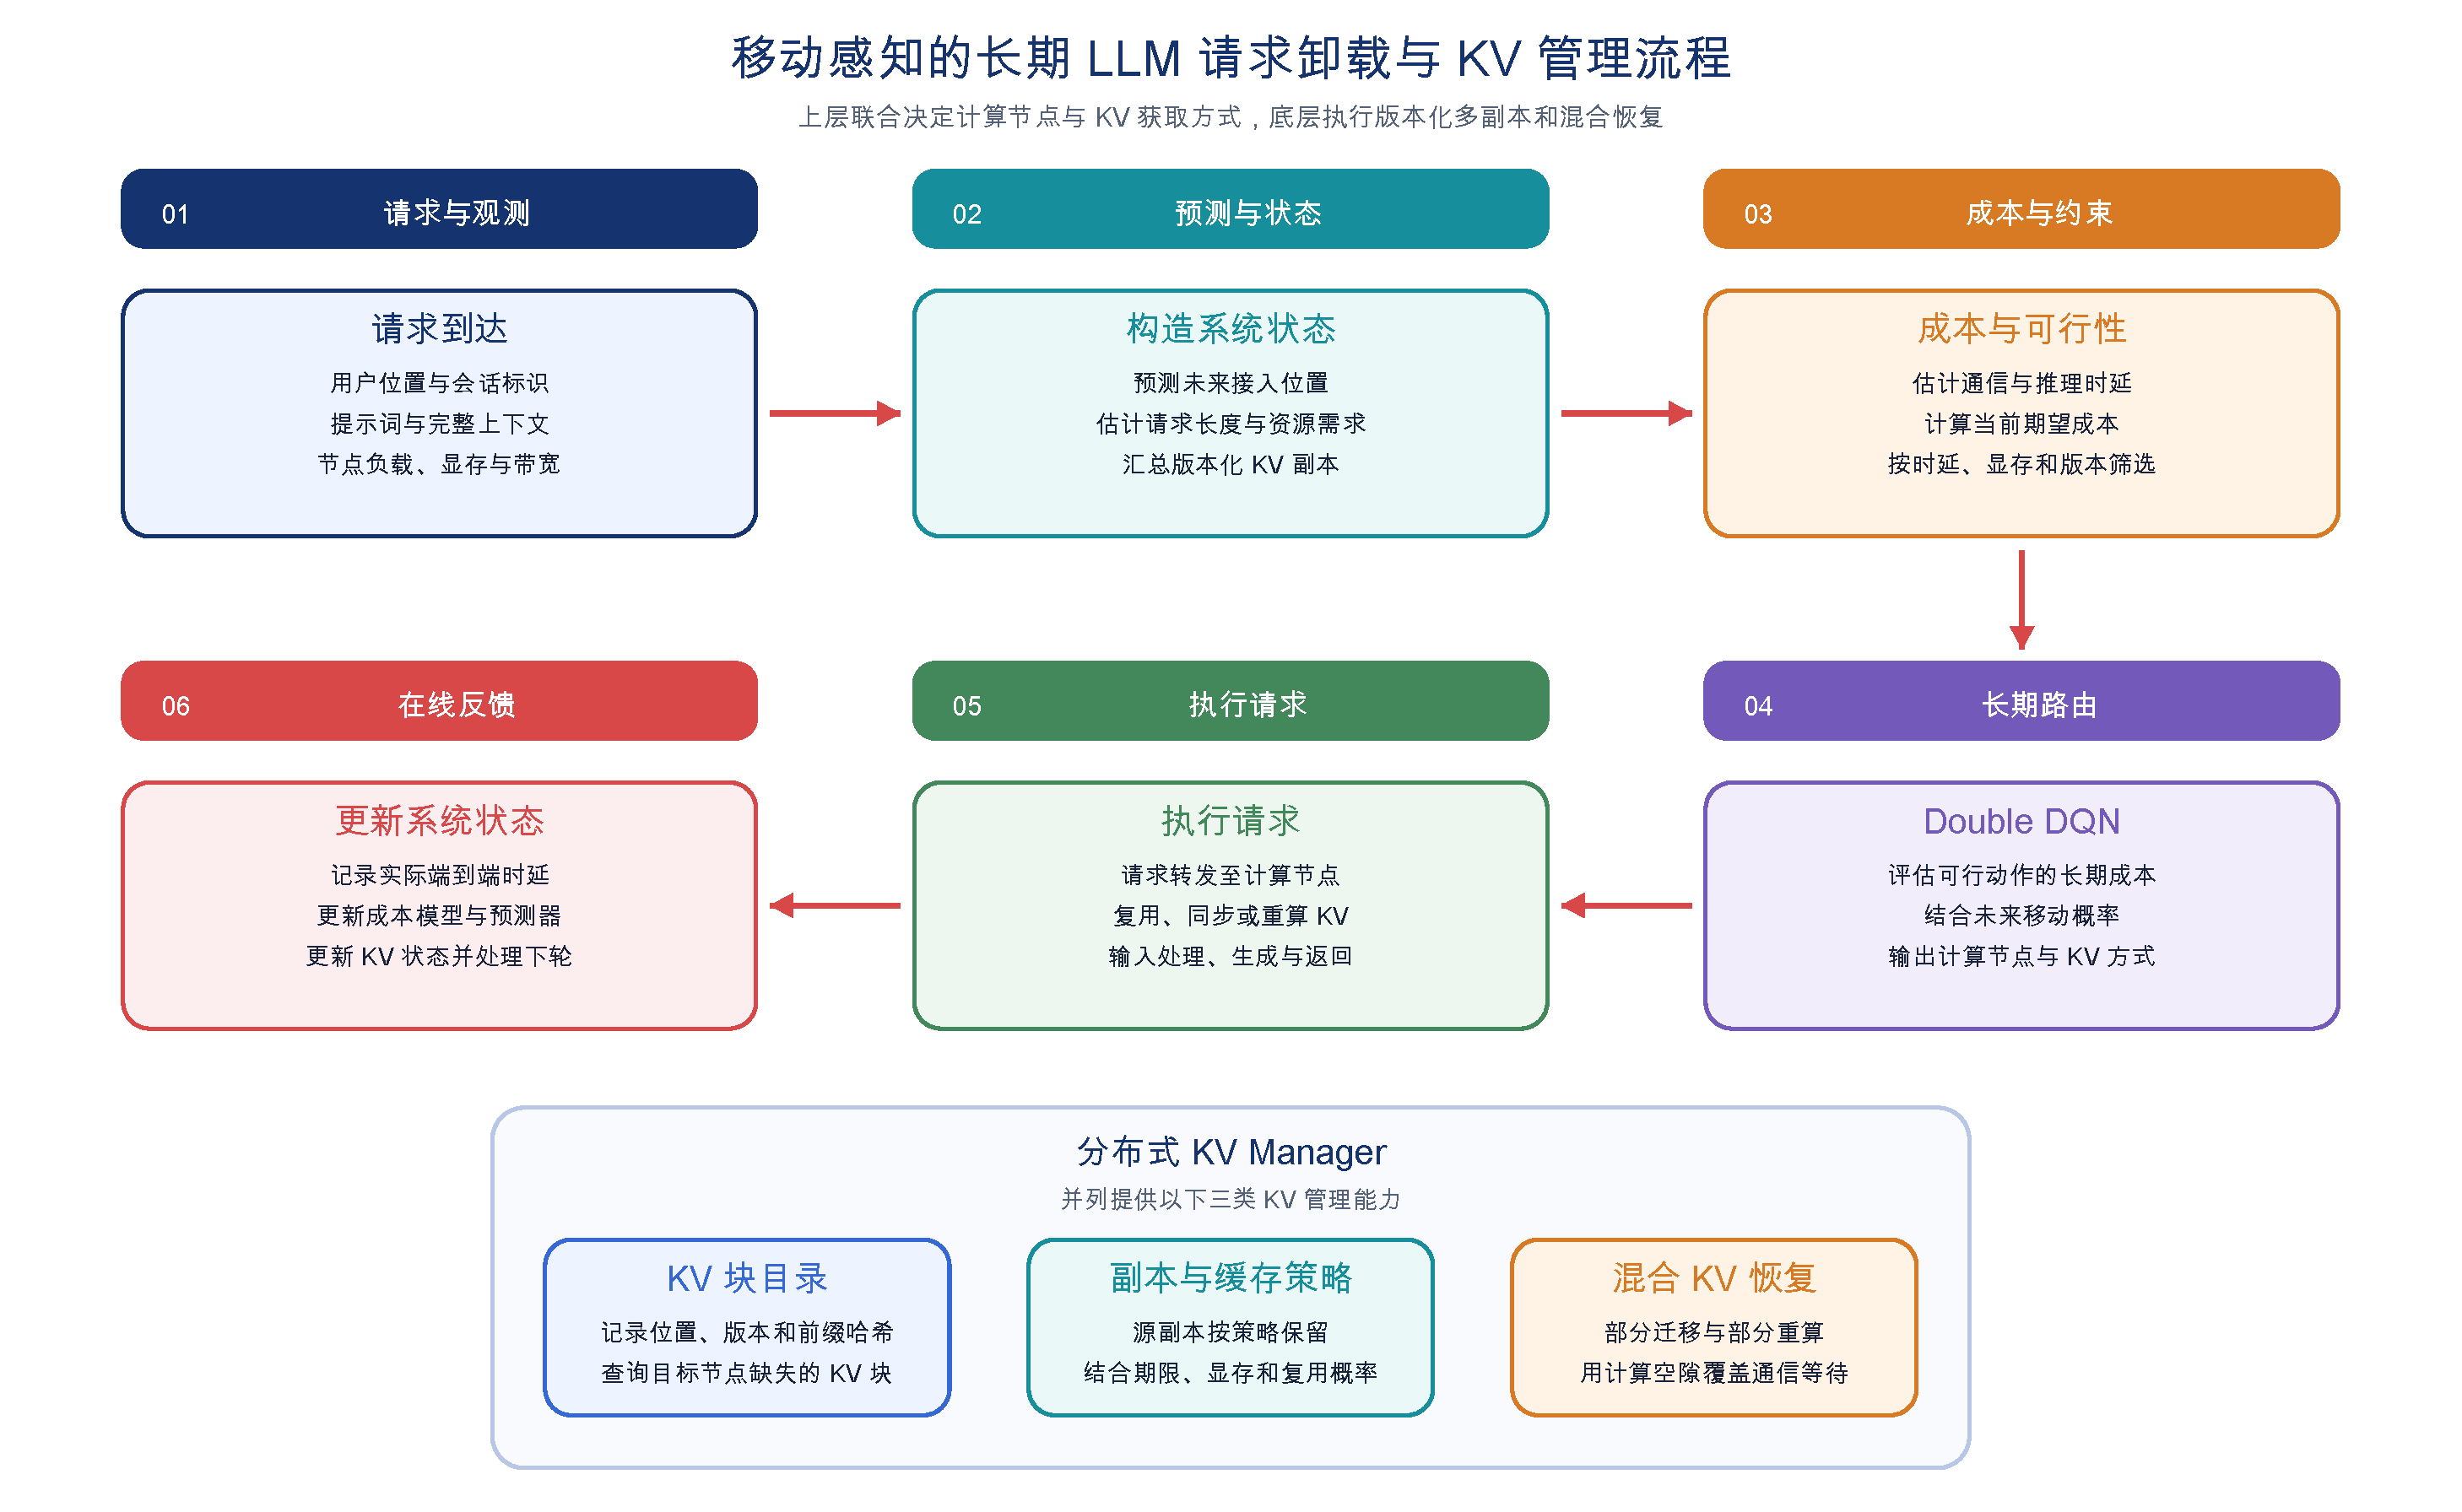
\includegraphics[width=\textwidth]{figures/ch6_mobility_offloading_workflow.pdf}
\caption{\textbf{面向用户移动的长期 LLM 请求卸载与 KV 管理流程。}上层路由器联合选择计算节点与 KV 获取方式，底层 KV manager 负责版本化多副本、缓存管理以及部分迁移与部分重算的混合恢复。}
\label{fig:ch6-mobility-offloading-workflow}
\end{figure}

\textbf{移动、长度与 KV 状态。} 令 \(U_k\in\mathcal N\) 为第 \(k\) 个请求的入口节点，移动模型给出
\[
P_{ij}(\Delta\tau_k)
=
\Pr(U_{k+1}=j\mid U_k=i,\Delta\tau_k).
\]
固定请求间隔时可采用 Markov chain，间隔变化较大时可采用 continuous-time 或 semi-Markov 模型；LSTM 或 Transformer 则输出多步入口分布 \(b_k\)。这一设计借鉴 MGCO 对历史决策和未来移动状态的利用 \refcite{61}。输出 token 数 \(Y_k\) 在决策时未知，由预测器给出 \(\rho_k(y)=\Pr(Y_k=y\mid x_k)\)；类似的长度预测已用于不可预测请求调度 \refcite{56}。长度预测仅用于当前请求的 E2E latency 和显存需求估计。

KV 允许存在多个版本化副本：
\[
\mathcal C_k
=
\{(n,v_{k,n},\mathcal B_{k,n})\mid n\in\mathcal N\},
\]
其中 \(v_{k,n}\) 和 \(\mathcal B_{k,n}\) 分别表示节点 \(n\) 的最高连续版本和 block 集合；节点 \(j\) 缺失的 blocks 为 \(\mathcal M_{k,j}=\mathcal B_k\setminus\mathcal B_{k,j}\)。同步后不默认删除源副本，保留或驱逐由 cache policy 决定。

\textbf{联合动作。} 动作定义为
\[
a_k=(J_k,Z_k),\qquad
Z_k\in\{\mathrm{reuse},\mathrm{sync},\mathrm{recompute}\},
\]
其中 \(J_k\) 是计算节点，\(Z_k\) 是该节点获取 KV 的方式。若 \(U_k\ne J_k\)，请求自动转发；存在多个副本时，系统自动选择同步时间最短的源节点。例如 KV 在 A、用户当前位于 B，但预测其即将到达 C，策略可以选择 \((C,\mathrm{sync})\) 或 \((C,\mathrm{recompute})\)，使当前请求直接在 C 执行。请求完成后的状态转移为
\[
\mathcal C_{k+1}
=
G(\mathcal C_k,a_k,\Delta\mathcal B_k,\psi_k^{\mathrm{cache}}).
\]

\textbf{成本与约束。} 请求通信、KV 状态准备和 prefill 时间分别为
\[
T_k^{\mathrm{comm}}(a_k)
=
\mathbf{1}\{U_k\ne J_k\}
\frac{D_k^{\mathrm{input}}}{BW_{U_k,J_k}^{\mathrm{eff}}},
\]
\[
T_k^{\mathrm{state}}(a_k)
=
\left\{
\begin{array}{ll}
\displaystyle
\frac{\sum_{b\in\mathcal M_{k,J_k}}q_b}
{BW_{s,J_k}^{\mathrm{eff}}},
&Z_k=\mathrm{sync},\\
0,&Z_k\in\{\mathrm{reuse},\mathrm{recompute}\},
\end{array}
\right.
\]
\[
T_k^{\mathrm{prefill}}(a_k)
=
\left\{
\begin{array}{ll}
\tau_{J_k}^{\mathrm{prefill}}(L_k^{\mathrm{new}}),
&Z_k\in\{\mathrm{reuse},\mathrm{sync}\},\\
\tau_{J_k}^{\mathrm{prefill}}(L_k^{\mathrm{ctx}}),
&Z_k=\mathrm{recompute}.
\end{array}
\right.
\]
其中 \(\tau_{J_k}^{\mathrm{prefill}}(L)\) 是节点 \(J_k\) 处理 \(L\) 个 prefill tokens 的实测时间；因此 recompute 会处理完整 context，而 reuse/sync 只处理尚未被 KV 覆盖的新输入。完整请求时延为
\[
\begin{array}{rl}
T_k^{\mathrm{E2E}}
={}&T_k^{\mathrm{comm}}+T_k^{\mathrm{queue}}
+T_k^{\mathrm{state}}+T_k^{\mathrm{prefill}}\\
&+T_k^{\mathrm{decode}}(Y_k)+T_k^{\mathrm{return}}(Y_k),
\end{array}
\]
它已经包含首 token 响应阶段。由于输出长度未知，决策时的即时成本定义为
\[
c_k(s_k,a_k)
=
\mathrm E_{Y_k\sim\rho_k}
\left[
w_1T_k^{\mathrm{E2E}}(s_k,a_k,Y_k)
+w_2D_k^{\mathrm{request}}(a_k,Y_k)
+w_3D_k^{\mathrm{KV}}(a_k)
+w_4C_k^{\mathrm{eviction}}(a_k)
\right].
\]
其中 \(T_k^{\mathrm{E2E}}\) 衡量完整请求时延；\(D_k^{\mathrm{request}}\) 是入口与计算节点不同时传输的输入及输出字节数；\(D_k^{\mathrm{KV}}\) 是为当前动作同步的 KV 字节数；\(C_k^{\mathrm{eviction}}\) 是驱逐仍可能复用的 blocks 所造成的价值损失。权重 \(w_1,\ldots,w_4\) 用于完成单位归一化并反映时延、带宽和缓存损失的重要性。若训练环境已通过后续状态精确体现驱逐代价，则令 \(w_4=0\)，避免与长期价值重复计费。请求完成后，系统用实际 \(Y_k\) 和实测开销生成 replay 样本。

系统使用输出长度高分位预测 \(\widehat Y_k^{(p)}\) 构造可行动作集合
\[
\mathcal A_k^F
=
\left\{
a:
\widehat T_k^{\mathrm{E2E}}(a,\widehat Y_k^{(p)})+\Delta_k(a)\le SLA_k,\quad
\widehat M_k(a,\widehat Y_k^{(p)})+M^{\mathrm{reserve}}\le M_{J_k}^{\mathrm{free}}
\right\},
\]
并检查 KV 版本和节点可用性。高分位预测用于降低输出长度低估造成的 SLA violation 与显存不足。

Greedy baseline 仅在可行动作中选择当前成本最低者：
\[
a_k^{\mathrm{greedy}}
=
\arg\min_{a\in\mathcal A_k^F(s_k)}c_k(s_k,a).
\]
它能够响应当前负载和链路状态，但不考虑本次同步或重算对后续 KV 复用的影响，因此作为本文长期策略的短视对照，也作为 RL 异常时的安全回退。

\textbf{长期优化。} 将第 \(k\) 个请求到达时的状态写为
\[
s_k=
(k,U_k,b_k,\rho_k,\mathcal C_k,\mathbf L_k,\mathbf M_k,\mathbf W_k),
\]
分别描述入口及其预测、输出长度分布、KV 状态、负载、显存和链路。有限时域优化问题为
\[
\begin{array}{ll}
\displaystyle\min_{\pi}\quad&
\displaystyle
\mathrm E_{\pi,U}
\left[\sum_{k=1}^{K}\gamma^{k-1}c_k(s_k,a_k)\right]\\
\mathrm{s.t.}\quad&
a_k=\pi(s_k),\quad a_k\in\mathcal A_k^F(s_k),\\
&U_{k+1}\sim P(\cdot\mid U_k,\Delta\tau_k),\\
&\mathcal C_{k+1}
=G(\mathcal C_k,a_k,\Delta\mathcal B_k,\psi_k^{\mathrm{cache}}).
\end{array}
\]
其中 \(c_k(s_k,a_k)\) 已对当前输出长度取条件期望。对应的理论最优状态--动作价值满足
\[
\begin{array}{rl}
\mathcal Q^*(s_k,a_k)
={}&c_k(s_k,a_k)\\
&\displaystyle
+\gamma\sum_{u'\in\mathcal N}
P_{U_ku'}(\Delta\tau_k)
\min_{a'\in\mathcal A_{k+1}^F(s_{k+1}(u'))}
\mathcal Q^*(s_{k+1}(u'),a').
\end{array}
\]
移动性既影响当前转发成本，也通过 \(P_{U_ku'}\) 影响未来价值；当前动作改变 KV 分布，所以优化对象是整个 session，而非单次最低时延。这延续了 QoS-LLM-Router 的长期 QoS 优化 \refcite{55} 和 MGCO 的非短视移动卸载思想 \refcite{61}，并将 CA-AIGC-Migration 的移动 context 管理 \refcite{69} 细化到版本化 KV blocks。

\textbf{动作掩码 Double DQN。} 上式定义了希望逼近的 \(\mathcal Q^*\)。对短 session、离散状态且已知真实轨迹的小规模实验，可用有限时域动态规划或搜索得到离线 oracle；一般场景一个session的request数量不确定，存在动作序列和状态爆炸，因此采用 Dueling Double DQN 近似求解。DQN 对所有固定动作输出 Q 值，在执行 \(\arg\min\) 前将 \(a\notin\mathcal A_k^F\) 的 Q 值置为 \(+\infty\)；训练和在线决策使用同一 mask，从而避免选择显存、版本或节点条件不满足的动作。

Double DQN 对每个可能的下一入口 \(u'\) 先用在线网络选择动作，再用目标网络评价：
\[
\begin{array}{rl}
a_{k+1}^{\mathrm{sel}}(u')
={}&\displaystyle\arg\min_{a'\in\mathcal A_{k+1}^F}
\mathcal Q_\theta(s_{k+1}(u'),a'),\\
V_{k+1}(u')
={}&\mathcal Q_{\bar\theta}
(s_{k+1}(u'),a_{k+1}^{\mathrm{sel}}(u')),\\
z_k
={}&c_k(s_k,a_k)
+\gamma\displaystyle\sum_{u'\in\mathcal N}
P_{U_ku'}(\Delta\tau_k)V_{k+1}(u').
\end{array}
\]
即训练目标等于“当前成本 + 折扣后的期望未来成本”，在线动作则为 \(a_k^*=\arg\min_{a\in\mathcal A_k^F}\mathcal Q_\theta(s_k,a)\)。若模型异常则回退至可行动作中的 Greedy 方案；若集合为空，则排队、降级或拒绝。

\textbf{分布式 KV 管理。} 借鉴 Mooncake 的 KVCache-centric 全局存储思想 \refcite{21}，系统建立分布式 block directory，记录 model/adapter 版本、prefix hash、token 区间、block 版本、大小和所在节点。执行 \(\mathrm{sync}\) 前，目标节点先查询已有 blocks，系统根据 \(\mathcal M_{k,J_k}\) 选择一个或多个源节点，并将缺失部分直接传至计算节点；这也吸收了 prefill/decode 分离系统中 KV handoff 的思路 \refcite{7}。同步不等于删除：源 blocks 继续保留，直至 cache policy 根据 TTL、显存压力、未来入口与复用概率、增量同步收益和重建成本决定驱逐。

KV manager 还可以在不扩大 RL 动作空间的情况下，把一次 \(\mathrm{sync}\) 细化为“部分迁移 + 部分重算”。在依赖关系允许时，将缺失集合划分为
\[
\mathcal M_{k,J_k}
=
\mathcal M_{k,J_k}^{\mathrm{mig}}
\mathbin{\dot\cup}
\mathcal M_{k,J_k}^{\mathrm{rec}},
\]
其中前者从其他节点传输，后者从目标节点已有的连续 prefix/checkpoint 开始重算。迁移与重算按 block 流水并行，使计算 bubble 尽量覆盖通信 bubble；理想情况下，状态准备时间由二者之和降为接近
\[
T_k^{\mathrm{hybrid}}
\approx
\max\{T_k^{\mathrm{mig}},T_k^{\mathrm{rec}}\}
+T_k^{\mathrm{overhead}},
\]
同时实际传输量只包含 \(\sum_{b\in\mathcal M_{k,J_k}^{\mathrm{mig}}}q_b\)。因此该机制既可能缩短状态准备时间，也能减少 KV 带宽使用；具体划分由 block 依赖、计算余量、链路带宽和显存水位共同决定。启用该机制时，KV manager 用实测 \(T_k^{\mathrm{hybrid}}\) 和实际迁移字节数替换基础全量同步估计，但上层动作仍保持 \((J_k,\mathrm{sync})\)。由此，Mooncake 的集群级 KV 管理被扩展为面向用户移动的版本化多副本与混合恢复管理。

\textbf{在线闭环与实验。} 请求完成后，系统用实际输出长度、E2E latency、KV 增量、传输量和显存变化更新长度/移动预测器、成本模型与 replay buffer。

主对比设置就近路由、当前成本 Greedy 和本文 RL 三种策略；补充实验只增加“全程无移动”对照，以及 10\%/20\%/30\% 改发比例的敏感性分析。核心指标为 SLA 下最大并发数、平均/P95 E2E latency 和 SLA violation；KV 传输量、prefix/block 命中率、同步/重算次数与显存峰值仅用于解释结果。

\phantomsection
\subsection*{6.5 小结}
\addcontentsline{toc}{subsection}{6.5 小结}

总体来看，CEC 中的 LLM inference task offloading 已超出传统“数据量、CPU cycles 与 deadline”驱动的节点选择问题。系统既要路由完整请求和连续 session，也要编排多模型/多 agent workflow，并管理 context、prefix cache、KV cache 和 agent memory。用户移动进一步改变请求入口、网络路径和历史状态位置，使一次卸载动作持续影响后续多轮服务。

现有研究呈现三条主线：request/session routing 从就近执行转向质量、SLA、队列和显存联合感知；multi-model/multi-agent orchestration 从单模型选择扩展到角色、模型、工具和中间状态的跨节点编排；runtime-state management 则将 KV 和 context 视为可驻留、复制、同步、驱逐或重算的系统资源。三者共同表明，LLM 卸载需要从 computation-aware 走向 computation-state co-optimization。

面向项目场景，本章构建“状态同步--长度与移动预测--显式可行性过滤--RL 长期路由--block-level KV 管理--在线反馈”的闭环。移动概率和输出长度分布共同进入未来成本估计；KV 状态由各节点的 blocks 与版本共同描述，同步后是否删除源副本由 cache policy 决定。动作掩码 Double DQN 在满足 SLA、显存和版本一致性的候选中，联合选择计算节点与 reuse、sync 或 recompute 方式，从而避免 Greedy 策略的状态黏附和无效数据移动。

后续工作可进一步研究请求执行期间 handover、多用户资源竞争、prefill/decode 分离和 CEC-native agent workflow，并探索移动与输出长度预测同卸载 regret 的联合训练。由此，CEC 中的 LLM inference offloading 将从单次执行位置选择发展为面向请求、workflow 和版本化运行时状态的长期协同优化。
